\documentclass[12pt,a4paper,titlepage,oneside]{scrartcl}
\newcommand{\lang}{en}
\usepackage{gaborProtocol}

\newcommand{\datum}{\today}
\newcommand{\lvaname}{Seminar aus Medizinischer Informatik}
\newcommand{\lvanr}{188.948}
\newcommand{\semester}{SS 2017}
\newcommand{\colormode}{color}
\newcommand{\dokumenttyp}{Image Encryption in Medicine}
\usepackage{xcolor}
\usepackage{amsmath}
\usepackage{siunitx}
\usepackage{float}
\newcommand\todo[1]{\textcolor{red}{#1}}

\begin{document}
\maketitle
\setcounter{section}{0}
\setcounter{tocdepth}{2}
\tableofcontents
\newpage

\section*{Abstract}
In this paper we analyze the problem which arises from the lack of security and privacy provided by DSLR cameras.
Especially in the fields of medicine and journalism a high level of the previously mentioned properties is required.
This state of the art report provides a detailed overview of the current approaches in science.
We analyze the approaches by four specific properties defined in this paper: the speed of the encryption in MB/s, the universality how the solution may be used, the quality of the implemented encryption algorithm and the possibility of plausible deniability.
These properties are compared in order to determine the best practice in the state of the art.
Our research results in four different approaches for the statement problem, where none satisfies all of our requirements.
In the discussion, we aim to give a direction of where a best practice approach could lead to in the future.

\newpage
\section{Introduction}

Privacy is one of the key issues of the information age.
Especially in the post-Snowden era this fact has become clear to the most individuals around the globe. 
Numerous regulations and laws \cite{EHG2015, DSG2000, ELGA2012, EuropeanParliament2016, EuropeanCourtofHumanRights2010} require it across all kinds of use cases and industries.
A well known way to achieve privacy is through encryption, which means encoding an information in such a way that only authorized parties can access it. 
Hardly any efforts on implementing encryption can be found in photography, which is a remarkable finding, keeping in mind that photographs are generally among the most private media.
This statement becomes even more astonishing considering the year, when the first patent for such a solution was registered: 1999. \cite{steinberg1999method}
To fulfill the requirements of privacy in photography it might be necessary to encrypt photographs right after they are taken.

Especially in the context of medicine this is very important as health data is considered the most private data. \cite{williams2013}
Medical photographs show a patients body, they are used to document visual properties of the skin, the state of a wound or the progress of a plastic surgery. 
All of the above mentioned photographs document very private information about an individual, which is only to be seen by authorized persons.
Theft of such photographs would have a dramatic impact on the patients privacy.

Another important application for encryption of photographs is journalism.
Journalists are looking for possibilities to hide any traces of sensitive material on their devices, for obvious reasons.
This is called ``plausible deniability (pd)'', or to be more precise, according to the Oxford dictionary, plausible deniability is ``the possibility of denying a fact, especially a discreditable action without arousing suspicion''.\cite{OxforddictPlausibleDen}
Journalists take big risks on them when taking precarious pictures in countries with authoritarian governments, where such actions are considered as act of crime and punished with imprisonment or even death penalty \cite{Amnesty2016}.
So it could be possible that encryption would not be enough to keep the journalists safe, as a trace of encrypted images could already lead to punishments.
Encryption is a first step to achieve this level of privacy.
For this reason 150 journalists wrote an open letter to camera manufacturers, asking them to implement such a feature, in December 2016.\cite{fp2016}

So we can state that there is a demand for digital single-lens reflex (DSLR) photo encryption feature which is not (yet) satisfied by state of the art devices.
This fact may lead physicians or journalists to take their private devices, which support encryption, for taking photographs, which is no real option for neither professional privacy nor professional image quality.

Privacy is strictly regulated by law, the most important regulations may be found in the general protected data regulation of the EU \cite{EuropeanParliament2016}, the European convention of human rights \cite{EuropeanCourtofHumanRights2010} or the respective national law. \cite{EHG2015, DSG2000, ELGA2012}

Another issue that may  be stated here is that even if custom solutions for encryption do exist, they are not implemented to be turned on and off again easily.
This leads to the conclusion that it is not possible to perform image encryption without a required amount of previous knowledge and expertise with such solutions.

Our goal is to evaluate different possibilities, to make on-the-fly encryption for DSLR cameras possible.
To ensure comparability between the introduced possibilities it is inevitable to define measurable parameters.

As encryption requires computational resources, its performance is dependent on the platform it is used on.
Considering this fact it is essential to be aware of the limited hardware resources of DSLRs that can be used for encryption.
So we can state that the performance of the implemented algorithm may be measured by the speed of the encryption process (v\textsubscript{encryption}).
Furthermore, a threshold must be found that determines the minimal speed (v\textsubscript{min}) of the encryption process.

Additionally, it must be assured that the encrypted information may only be decrypted by authorized persons.
For this reason, the used encryption algorithm must be considered safe, according to the state of the art.

To ensure a specific degree of performance it is necessary that the evaluated solution does rely on as little proprietary soft- and hardware as possible.
An important information which is not known to us for now: whether or not it is better to perform encryption on DSLRs with software or hardware.
In the first place, this is a performance related topic, but it has big impact on portability.

Our final goal is to create a method which can evolve to a best practice, which gives the medical and journalist community the possibility to protect their data with the help of encryption.
A best practice solution should fulfill the following requirements in the best possible way.
\begin{enumerate}
  \item The speed of the encryption process must be greater than the defined threshold (v\textsubscript{encryption} $\geq$ v\textsubscript{min});
  \item The used encryption algorithm must be considered safe.
  \item The solution must not be limited to one DSLR manufacturer.
  \item Plausible deniability must be assured.
\end{enumerate}

\subsection{Encryption}
As in this document we write about solutions, which use encryption, that is why we provide the reader some basic information about encryption.
According to the Oxford Dictionary encryption is the process of converting information or data into a code with the goal to prevent unauthorized access. \cite{OxforddictEncrypt}

In the field of cryptography there are two ways to encrypt something.
Either asymmetric or symmetric encryption algorithms can be used.
The main difference in the two methods are, that in case of the asymmetric encryption two keys are being used.
One for the encryption and a second one for the decryption.
On the other hand in case of the symmetric encryption there is only one key used both for the de- and encryption.
As we, during our project, mostly used symmetric-key schemes, we focus on this, and we will not write about public-key schemes.

There are two major groups of symmetric encryption algorithms.
These are the block- and stream ciphers, where cipher refers to an algorithm to perform encryption or decryption.
Block cipher algorithms divide the data into equal size blocks, and with the help of the encryption-key they perform the encryption on each block individually.
Stream ciphers are a special kind of block cipher, where the block size is one byte. \cite{menezes1996handbook}
Further classification of block- and stream ciphers will not be included, as it would go beyond the scope of this paper.

\subsubsection{Advanced encryption Standard}
The currently wildly used algorithm for encryption is the Advanced encryption standard (AES), which was defined in 2000, to replace the previous one, which was considered insecure.

AES uses the Rijndael algorithm with some restrictions.
Rijndael was invented by Daemen et. al. \cite{daemen2013design}

As Rijndael is a block cipher the round transformations will be applied on the data blocks in round number (N\textsubscript{r}) of times, which can either be plain text blocks or cipher blocks.
The input for the algorithm is the key and the plain text block, and the output is the cipher block, or the cipher block with the key, and the output is in this case the plain text block. \cite{daemen2013design}

First the algorithm derives the round key from the user key, which will be used during the initial key addition.
After this, the round transformations will be applied N\textsubscript{r}-1 times, and finally during the final round the encryption is considered done.
One round consists of four transformations,
\begin{labeling}{AddRoundkey}
\item [SubBytes] This is the only non-linear transformation of the algorithm. Every byte will be mapped on an other with the help of a Substitution-Box (S-Box).
\item [ShiftRows] During this step every row of the state (which is a 2D-array representation of the block) will be shifted cyclically over different offsets.
\item [MixColumns] In this step every column will be multiplied by the following polynomial \begin{math} c(x) = 03 * x^3 + 01 * x^2 + 01 * x + 02 \mod x^4 + 1 \end{math}
\item [AddRoundkey] In this final step we apply bit-wise XOR to the current block with the round key.
\end{labeling}
The decryption uses the inverse of the round transformation, which means they do the same, only in the other direction. \cite{daemen2013design}

\subsubsection{ChaCha}
Without going into too much detail, we are shortly going to introduce the ChaCha encryption algorithm, as we are going to use it later.

ChaCha is a derivative of the Salsa20 algorithm family. 
The Salsa20 algorithm is a stream cipher, so according to our previous definition by Menzenes et al. in \cite{menezes1996handbook} we are talking about a cipher where the block size is one byte.
However according to Bernstein, Salsa20 ``generates the stream in 64-byte blocks''. \cite{bernstein2008salsa20}

But without being caught up too long with the categorization of an algorithm lets jump to the description of how Salsa20 and ChaCha work.
Salsa20 uses a 256-bytes key, which will be expanded with a 64-bit unique message number to a \begin{math} 2^{70} \end{math}-bytes stream.
To encrypt \textit{b}-byte of plain text (where b is an integer) it takes the first \textit{b}-bytes of the stream and XORs it with the plain text.
The rest of the stream will not be used.
The decryption works just like the encryption.
Salsa20 works only with 3 kind of operations on 32-bit words.
These are addition of two numbers modulo \begin{math} 2^{32} \end{math}, XORing two numbers and rotating a number by some constant bits.
These three operations can be run on every CPU very efficiently, without needing and dedicated hardware like in the case of AES. \cite{bernstein2008salsa20}

ChaCha, as mentioned before is a derivative of the Salsa20-family.
There are three differences:
\begin{enumerate}
  \item Due to performance effects the order of the words within the output block are permuted.
  \item The initial matrix which is used during the encryption and decryption is built in a slightly different way.
    In the case of Salsa20 the user inputs are scattered within the matrix, whereas in ChaCha these reside in the last row of the matrix.
  \item ``ChaCha sweeps through the rows in the same order in every round.''
\end{enumerate}
\cite{bernstein2008chacha}

\newpage
\section{Method}
The aim of this chapter is to describe the methodology used when performing the research for related literature on the topic of this paper.
Several search strategies have been used in order to get as much relevant literature as possible.
Relevant literature includes all kinds of scientific papers, conference proceedings, master's and bachelor's thesis covering topics around encrypting and hiding photographs.

The most handy tool in order to filter out relevant literature was Google scholar. 
Also Institute of Electrical and Electronics Engineers (IEEE) Xplore turned out to be a good and reliable source for state of the art literature in the selected field.
To satisfy the medical aspect of the problem statement it was inevitable to use the pubmed database search engine of the National Center for Biotechnology Information (NCBI).
Furthermore, the CatalogPlus of the TU Wien, turned out to be a reliable tool when it comes to filtering out scientific valuable content.
The following keywords were used in order to get relevant search results:
\begin{enumerate}
  \item  \textbf{encryption, cryptography, crypto}
  This keywords were used to assure that the topic of the found literature correlates to aspects of cryptography.
  \item  \textbf{medicine, medical}
  As the search results may include application in the field of medicine these keywords can be used.
  \item  \textbf{journalist, journalism}
  To receive search results that stand in relation to journalism these keywords may be used.
  \item \textbf{camera, digital camera, DSLR}
  As lots of papers discuss the encryption of images on convenient PCs, these keywords are necessary to filter for the application of cryptography on such devices.
  \item \textbf{deniable encryption, plausible deniability sd card}
    There were considerably lower amount of papers related to plausible deniability in case of flash drives, that we had suspected.
\end{enumerate}

In the context of medicine it was important to filter out results that are only related to medical imaging techniques like MRI.
This is not because this research is limited to the content of the image recorded, but rather to the device, the image was captured with.
For this reason, papers addressing issues in dermatology or wound management were considered relevant as these domains tend to use conventional image capturing devices.

Numerous papers were found regarding the issue of watermarking.
Watermarking, in this context, describes the process of modifying an image so it is possible to identify source, creator or owner of a photograph.
So we can state, that watermarking addresses issues in the field of integrity but does not provide any advantage in terms of confidentiality, as it is required by the topic of this paper.

The result of the above mentioned research is a set of relevant literature that marks the state of the art in the topic of this very scientific work.
All in all it was possible to obtain four papers that mark the state of the art.

\newpage
\section{Results}
At this point, we have obtained all the papers that are valuable for our research.
In the following sections, the results of our research are discussed and even more importantly, compared to each other.
The state of the art in the selected topic is described by the entirety of the gained knowledge that is compressed in these results.
Furthermore, we will give a short overview of our comparison at the end of this chapter.

\subsection{Summary}
In this section we are shortly going to summarize the approaches found with our methodology.

The most outstanding work related to the topic examined in this state of the art report is titled ``A VHDL Architecture for Auto Encrypting SD Cards'' and was published by the University of Gothenburg in November 2016 \cite{Davidsson2016}.
To summarize, the students working on this master's thesis designed an encrypted SD-card for journalists.
The approach was based on a hardware solution.
An SD-Card adapter was designed, that applies to the SD-card standard, in other words, the auto-encrypting SD had the size and shape of a usual SD card.
Inside this seemingly normal SD-card there was an encryption hardware module, based around a FPGA and a publicly available intellectual property core, which was used for encryption.

Another approach to this issue, especially focused on plausible deniability was developed by Adam Skillen and Mohammad Mannan at the Concordia University in Montreal, Canada \cite{skillen2013implementing}.
This solution is basically an app (``Mobiflage'') that stores photographs on a deniable file system, which means hiding encrypted volumes within random data on the external storage of a mobile device.
The paper was published in 2013.
Google's Android operating system was used for the prototype implementation of Mobiflage.
Mobiflage features two modes for saving images: 
\begin{enumerate}
  \item Standard Mode
  In this mode the so called ``decoy'' password is entered at boot time and non-sensitive data is displayed.
  The storage medium is mounted as Mobiflage isn't installed.
  \item PDE mode
  In the PDE mode the user enters the ``trust'' password at boot time and the hidden data may be accessed on the SD-card.
\end{enumerate}

Similarly to Mobiflage another paper was identified that addresses the issue of secure storage of photographs on mobile devices.
Landman et. al \cite{pmid25565678} published a paper called ``A Mobile App for Securely Capturing and Transferring Clinical Images to the Electronic Health Record: Description and Preliminary Usability Study'' that describes an app developed for iOS devices called ``CliniCam''.
To enhance security, this app does not save the image permanently, it rather transfers it to a secure electronic health record (EHR) in PDF format.
The temporary storage of the photographs is handled within ``a secure temporary storage area allocated to the app'' this storage area is called sandbox.

For the file system we found the by Peters et. al. presented DEFY-file system solution.
DEFY stands for \textbf{D}eniable \textbf{E}ncrypted \textbf{F}ile System for \textbf{Y}AFFS.
YAFFS stands for \textbf{Y}et \textbf{A}nother \textbf{F}lash \textbf{F}ile \textbf{S}ystem.
The basic idea for DEFY is, that it defines different deniable layers, which have to be opened separately.
And as the whole file system is encrypted, an advisory can't find out if changes on the file system originate from some normal OS activity, or that the user tries to hide something.
Additionally they make sure, that if something gets deleted it is going to be erased from the drive. \cite{peters2015defy}

\subsection{Speed}
A critical factor for the quality of the solution is the speed of the encryption process.
This is the time between the capture and the secure storage of the image.
Images in the so-called RAW-format are the purest way of storing images, as the loss of quality through compression is minimized.
The size of a RAW photograph is highly depending on the quality of the used camera but is usually between 20MB and 50MB, so it might be necessary to wait quite a while for the encryption.
As already stated in the introduction the speed of the encryption process must be greater than the defined threshold (v\textsubscript{encryption} $\geq$ v\textsubscript{min}).
Davidsson et. al \cite{Davidsson2016} state in their paper that the transfer speed shall be at least 10MB/s.
As no other reliable source for the minimal speed requirement could have been found, this 10MB/s are considered state of the art.
As a results we can state that v\textsubscript{min} is 10MB/s.

We start with the analysis the approach of Davidsson et. al.
In their paper three bottlenecks are stated that define the speed of the encryption process.
The first one, the processor operation is stated to not affect the speed of the data transfer.
Secondly the encryption reaches a speed of 20MB/s and is therefore non critical for the success of the implementation.
Finally, the speed of the data transfer to the SD-card is mentioned, which does not meet our speed requirement.
This is caused by the used SPI interface, which has no official speed limit, but is said to `` often go over 10 Mb/s''\cite{leens2009introduction}.
So we can state that a bottleneck is in the best possible case slightly better than 10Mb/s which is way below our requirement of 10MB/s.

Mobiflage, the solution described by Skillen et. al \cite{skillen2013implementing} is hardware dependent.
The performance tests described in the paper were carried out on a Nexus S smartphone running Android 4.
The test conditions were as follows: 
Four files with sizes between 50MB and 200MB were written to the encrypted memory.
This process was repeated 20 times per file, resulting in an average writing speed of 5288$\pm$69KB/s.
Unfortunately, this value only reaches 50\% of the desired speed.

The analysis for CliniCam \cite{pmid25565678} is quite complex as the performance is not described in the paper.
As the image is not directly encrypted but rather just stored in the ``secure storage area'' and the storage is a highly performing NAND-flash, we can guess that the storage is not a bottleneck of the application.
As the image is not aimed to remain on the device, a transfer to the EHR server via WiFi is necessary.
The issue here is that this process must be started manually, which decreases the speed of the overall operation.
If a device with the 802.11ac standard is used, a speed of around 35MB/s may be reached, which is sufficient for our requirement.

Peters\cite{peters2015defy} provides two benchmarks for the speed analysis of DEFY: IOZone and FFSB.
The results of IOZone are displayed by Peters in figure~\ref{fig:iozone} where we can see that DEFY reaches \begin{math} 10^{4}-10^{5}\end{math} KB/s (or 10-100 MB/s) for write operation.
\begin{figure}[H]
  \centering
  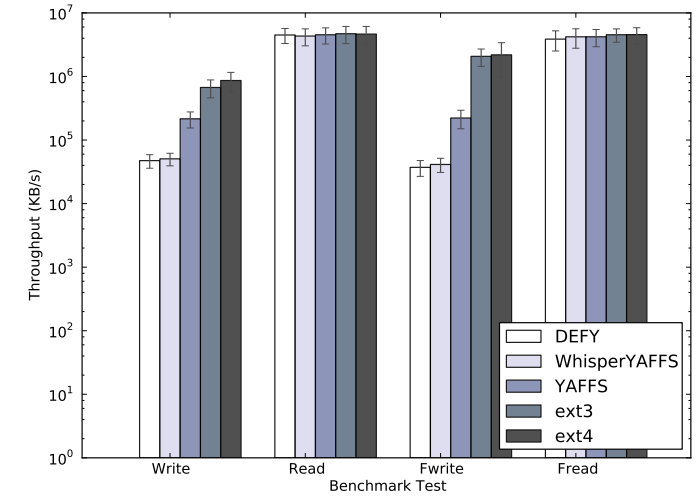
\includegraphics[width=\textwidth/9*8]{defy_figure_5_2.png}
  \caption{The performance of a number of file systems as measured by IOZone (note the log scale) \cite{peters2015defy}.} \label{fig:iozone}
\end{figure}
According to the results of the FFSB benchmark, shown by Peters in figure~\ref{fig:ffsb} DEFY manages a write operation speed of about 2500KB/s (2.5MB/s).
Unfortunately, these results are not very precise and fully disjunctive, as Mobiflage has a similar approach, the 2.5MB/s seem more realistic for a mobile devices memory.
\begin{figure}[H]
  \centering
  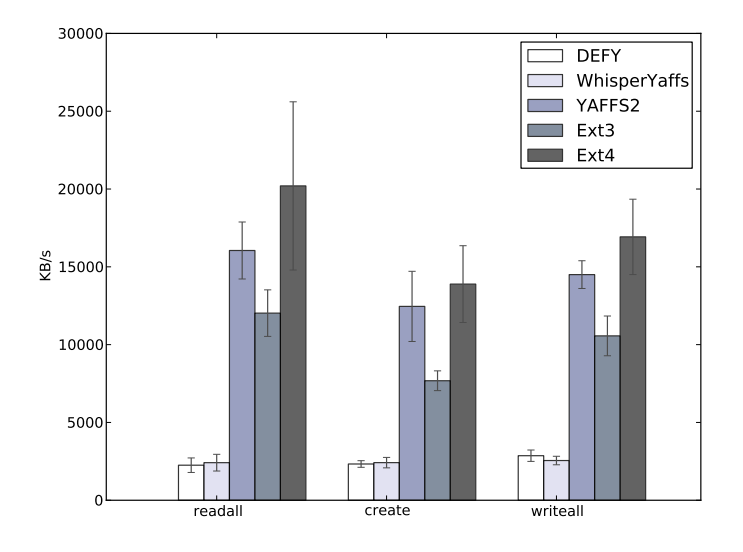
\includegraphics[width=\textwidth/9*8]{defy_figure_5_1.png}
  \caption{ The performance of a number of file systems as measured by FFSB\cite{peters2015defy}.} \label{fig:ffsb}
\end{figure}

\subsection{Universality}
As we can state for now there are plenty of possibilities to reach the target of professional photo encryption.
An issue that has to be aimed now is, whether the identified approaches are can easily be used across all kinds of use cases or not.
For this reason we will now take a look at the universality of the relevant attempts.

Davidsson et. al \cite{Davidsson2016} designed a solution that is based on a hardware platform.
This hardware platform is designed as SD-Card, not only in terms of size and shape this SD-Card is capable of communicating with all kinds of devices using an Serial Peripheral Interface (SPI) Bus.
So theoretically it would be possible to use this SD-Card in any digital camera, DSLR, PC or smartphone, that supports SD-cards.
A big problem here is the design as SD-Card, as the standard specification for smartphones is to use micro SD-Cards in order to keep this devices compact.

The approach of Skillen et. al \cite{skillen2013implementing} is the complete opposite in terms of design.
As this solution is designed as an Android app, it is of course limited to Android smartphones, with at least one micro SD-Card slot.
Considering that Android is the prevailing operating system for mobile devices Mobiflage is a promising application in terms of universality, at least for non-professional usage.
Anyway, porting this application for usage on professional DSLR devices will nearly be impossible unless the DSLR is powered by an Android powered operating system.

Similarly as the approach of Skillen, Landman et. al \cite{pmid25565678} deal with an approach that shows disadvantages in terms of universality.
This is caused by the single-platform design of the app CliniCam that allows it only to be executed on iOS platforms.
Another issue is that the platform iOS is bound to a single manufacturer, which makes CliniCam even more limiting.

As Peters approach \cite{peters2015defy} aims to design a file system, we can consider the universality to scale up for any kind of flash storage device.
On the other side, this file system must be supported by the given device.
What this means for DSLRs or smartphones will be discussed in the upcoming sections.

\subsection{Security}
As one of the crypto-algorithm which was used by us is by the NIST standardized, and still unbroken AES, and the other one is also a well tested algorithm, currently there should be no security issue regarding the cryptological strength of the used algorithm.
However for the sake of completeness, we will describe some key aspects of the security of the different solutions.

Rijndael was chosen by the NIST to be the new encryption standard, back in 2001.
Although some modes of encryption (like the ECB mode for more than one block) are considered week and insecure, the security which is provided by the algorithm remains unbroken.

As what Salsa20 and ChaCha considers, Salsa20 was one of the finalists of the ECRYPT Stream Cipher Project. \cite{bernstein2008salsa20}
Several papers reported, that they managed to break the encryption of Salsa20 or ChaCha if only 8 or less rounds were used. \cite{aumasson2008new, crowley2006truncated, fischer2006non, tsunoo2007differential}
But both ChaCha and Salsa20 are capable to work with up to twenty rounds, which even after twelve years after its submission to eSTREAM remains unbroken.

Keeping all this in mind, we can say, that the VHDL solution by Davidsson et. al. is considered secure, as they use a ChaCha20 implementation (this means ChaCha with 20 rounds). \cite{Davidsson2016}

In their solution Skillen et. al. uses AES in XTS mode.
XTS mode is commonly used for full disc encryption, and is also considered secure. \cite{alomari2014implementation}

The CliniCam paper provides no specific information about what kind of technology is being used.
The authors of the paper only say, that
\begin{enumerate}[label={\alph*}]
  \item ``The transmitted images are signed with the unique secret key of the user.''
    This indicates, that some kind of asymmetric crypto algorithm is used.
  \item ``The images are stored temporary in an encrypted area of the application memory.''
    This might indicate some symmetric crypto, however it would be interesting to know, where the key to this area resides.
    It is probably also in the memory, outside of the encrypted area, which makes the encryption area obsolete.
  \item ``Secure wireless transmission''
    The authors mention, that the transmission is only allowed through the secured WiFi network of the hospital.
    However they don't provide any information what kind of technology is used in this case, like if it is WEP or WPA/WPA2 or something else.
\end{enumerate}
All in all we categorized CliniCam in the point of security ``unknown'', as the authors didn't provide any specifics regarding the used technologies. \cite{pmid25565678}

To achieve encryption, Peters et. al use AES-CTR (AES in counter mode), which means as initialization vector a counter will be used. \cite{peters2015defy}

\subsection{Plausible deniability}
Denying the unauthorized access to information is relatively easy to achieve with encryption, encryption still doesn't solve the problem to hide the existence of the encrypted data.
As previously has been showed with choosing a strong enough key, cryptographic algorithms can act as a feasible protection, however, in some states the legislation can oblige the individuals to disclose their keys.
This means an advisory can often observe, that somebody tried to hide some information with the help of encryption, and maybe this advisory can even see the size or some other meta data of the file.
As it was reported in the news the former director of the NSA and CIA said, that they ``kill people based on meta data''. \cite{coleMetadata}
It is worth mentioning, that plausible deniability is only important in the context of journalism and not in the field of medicine.

To achieve plausible deniability we found two methods.
Either we solve the problem on the file system level, which means, we take a file system that allows to be configured in a way, where plausible deniability is possible, or we use deniable encryption.

The basic idea behind deniable encryption is, if the advisory acquires the cipher text and obliges the user to hand over appropriate key, then the user can hand over a fake key, which will lead to a biased decryption, which doesn't include any sensitive data, however the advisory can't tell if the decrypted information is fake or real. \cite{canetti1997deniable}
The problem is not that the decryption algorithm can't decrypt an information with a wrong key, because there are ways to configure the system in a way, that the algorithm doesn't check if the decrypted information is valid or not.
The problem is, like Trachtenberg describes, to create an output with a fake key, that will convince the advisory, that he got the real output.
Trachtenberg later describes in \cite{trachtenbergsay} a method how to implement deniable encryption based on the \textit{set reconciliation} in the context of strings.
However in our case this method is not really applicable, thus we have to handle specifically designed file formats, which even after decryption with a fake key should deliver a valid looking picture.

Davidsson et. al. provides plausible deniability by hiding the encrypted files within the file system.
This is performed by overlaying the original folder which stores the encrypted data with a copy within the FAT32 cluster sub region. \cite{Davidsson2016}

Mobiflage stores photographs on a deniable file system, which means hiding encrypted volumes within random data on the external storage of a mobile device.
Mobiflage achieves plausible deniability through plausible deniable encryption (PDE) this technique enables the output of different reasonable and innocuous plain texts from a given cipher text.
The original plain text (or the image data) is only revealed if the correct key is entered.
This makes the decrypted data seem correct for unauthorized individuals trying to force the disclosure of the encrypted information.
As Skillen et. al states, there is a file system for Linux called ``Rubberhose'' which features PDE.

Landman et. al \cite{pmid25565678} does not address the issue of plausible deniability at all, as this is out of scope for them.

As we already mentioned DEFY uses different multiple layers embedded into the file system.
This means each layer is encrypted with a different key, and the next layer is only disguised if the previous one got decrypted.
Additionally they use cryptographic deletion, which means, instead of actually deleting the encrypted block, they just permanently delete the key to it, which makes impossible to retrieve the data. \cite{peters2015defy}

\newpage
\section{Discussion}
In this section we are going to compare all of the detected approaches by the above defined parameters.
Table \ref{tb:overview} shows a short comparison of all approaches compared to each other.
Furthermore we are going to discuss advantages and disadvantages of the described methods.
Additionally we will point out which solution is commonly used and which is considered best practice for our problem statement.

\begin{table}[H]
   \begin{center}
     \begin{tabular}{| l | c | p{3cm} | c | c |}
     \hline
      \textbf{Approach}   & \textbf{Speed} & \textbf{Universality}                         & \textbf{Security} & \textbf{PD}                    \\  \hline
      Davidsson (FPGA SD) & >1.25MB/s      & all devices supporting SD cards               & ChaCha20          & \checkmark                     \\  \hline
      Skillen (Mobiflage) & app. 5.288MB/s & Android devices supporting SD cards           & AES-XTS           & \checkmark                     \\  \hline
      Landman (CliniCam)  & n/a            & iOS devices                                   & n/a               & X                              \\  \hline
      Peters (DEFY)       & >2.5MB/s       & all memory devices support flash file systems & AES-CTR           & \checkmark                     \\  \hline
     \end{tabular}
   \end{center}
\caption{Overview of all examined approaches.}
\label{tb:overview}
\end{table}

\subsection{Speed}
As we can see in the overview table Davdisson reaches comparably lower speed.
This is because of the bottleneck on the SPI bus.
The SPI bus was chosen despite the speed limit to reach the desired size of the hardware implementation.
Anyway, a change of the used protocol could likely provide a significant increase of speed.

Skillen provided the most detailed research on the speed transfer, at the importance of the speed was known to the authors.
The 5MB/s are even though the best value of all researched approaches.

No benchmarking information for the speed of the overall process (including WiFi transmission) was given by Clinicam.
We can only state that the speed of the transmission is highly dependent on the capabilities of the WiFi connection.

A significant disadvantage in the discussion of Peters' approach is the completely different benchmark results.
This was not discussed in Peters' thesis, which is quite unfortunate as such an issue should be addressed further.

\subsection{Universality}
Roughly we can differentiate two approaches to our problem statement defined in the state of the art.
Firstly there are the app solutions by Skillen and Landman, which only work on Android respectively iOS.
Even though both operating systems are widespread it would be a big advantage to see an universal approach for this issue to enhance portability.
Unfortunately Clinicam does not support any kind of external images source, so storing professional images of DSLRs is not possible.
Concerning Mobiflage it is possible to import images manually and store them securely, so it would be possible to take the photograph with a DSLR and encrypt it.

The clear advantage of the approach of Davidsson et. al \cite{Davidsson2016} is that the SD-card may be used in any device, regardless of DSLR or smartphone.
As most DSLRs support SD cards this is a big advantage for the encryption on any kind of device, independent of the manufacturer.
Anyway, as Davidsson uses the SD-card standard and not the micro SD-card standard it is unlikely that it can be used on a smartphone device.

Finally we can discuss Peters' approach.
The big advantage of DEFY is its design as a file system, which creates the possibility for it to be used on any kind of flash storage.
On the downside, the manufacturer of the devices on which such a storage is used must assure support of DEFY, which is very unlikely for DSLR manufacturers to do.
Even if DEFY would be able to be run on a DSLR it is very unlikely that there is support for providing multiple encryption passwords.

\subsection{Security}
Although Landman et. al. describes an application which transports highly sensitive data, they don't provide any specific technical information, what kind of algorithm or technology they used.
The only information is, that their implementation is conform to the Health Insurance Protability and Accountability Act (HIPAA).
In order to discuss the security of this application more detailed, we would have needed additional technical information.

The remaining three proposed solutions in our results can be categorized as secure, as they all use unbroken and secure algorithms.
In case of the FPGA SD solution by Davidsson the use of ChaCha (stream cipher) is advantageous, because in this way they don't need any caching, which would have lead to additional hardware.
Peters as we already mentioned uses AES-CTR and additionally he uses a hash based message authentication code with the hash function SHA256 (HMAC-SHA256).
However it would have been more beneficial if they have used AES in GCM (Galois/Counter Mode), which builds upon the CTR mode and already includes an HMAC. \cite{mcgrew2004security}
Skillen et. al. used AES-XTS, which is favorable for whole disc encryption.

All in all the last three solutions considered secure, however the AES variants can be disadvantageous if there is no hardware support for AES, in which case this algorithm is very slow.

\subsection{Plausible deniability}
As we in the results sections already mentioned in case of medical applications PD considered irrelevant, we won't discuss the CliniCam solution.

In Davidssons work an issue that has not been addressed completely in our opinion is the plausible deniability.
Even though the proposed solution ``hides previously created encrypted files from the camera'', it is not assured that this file hiding is sufficient towards forensic analysis.

As what the remaining two concerns, we can state the both provide a sufficient level of plausible deniability.
The strategy is mainly different in these solutions, as Peters tries to disguise the data on different layers, whereas Skillen returns faked data in case of providing a wrong key.
It is relatively hard to decide which of the two is better in practical usage.

\newpage
\section{Conclusion}
At the end of this scientific work we can state, that there are different approaches existing in literature that aim to address the issue described in our problem statement.
What is lacking is a universal solution that features a full pipeline from support of all photography devices (DSLRs, digital cameras, smartphones, ...) to the securely and hidden storing the data on the memory.
A high performing solution must be developed in order to fulfill the defined speed requirements as this is critical for the practicability of the solution in real life application.

Even though the problem statement is not new and the demand in the public domain and the scientific community has been existing for years now, it is only now that the industry turns towards this problem scenario.
For example, an interesting approach was developed by a company called swissbit, where a very similar approach to Davidsson was implemented in the size of a micro SD card \cite{swissbit2017}, so it would fit in a smartphone as much as in a DSLR.

As what concerns the best practice that could be established in the industry, it is our belief that there is no other way as including an encryption feature in the firmware of cameras.
As high the demand for such a feature in the photography community may be it is, in our opinion, inevitable to provide a standardized approach for it.
This is the only way a secure and widespread standard can establish.
It must also be addressed how the encryption feature can be set up on a camera, where no full keyboard is available.

What we have learned in the course of our research is, that plausible deniability is everything but trivial.
There are several approaches from completely hiding the sensitive information to returning fake information if needed.
It is to be decided which approach is more applicable in a real life scenario.
Further research should be carried out in order to address this issue.
Another possible research field about this problem is to evaluate whether or not there is a possibility to create an open platform for flash memory encryption like Google's project vault.

\newpage

\listoffigures

\newpage

\listoftables

\newpage

% Add a bibliography.
\bibliographystyle{ieeetr}

\bibliography{star-report}
\end{document}
